\chap{Enhanced Generative Adversarial Network}

\section{Introduction}

\section{GAN Architecture} 

The original paper's\cite{Original-GAN} generator architecture consisted of  rectifier linear\cite{RELU} and sigmoid activations, while the discriminator net used maxout [10] activations. the results were good but lacked stability and also suffered from problem of model collapse.
Later, Radford \textit{et al.}\cite{DCGAN} proposed deep convolution generative adversarial network which used deep convolution with fractional stride convolution and batch normalization to stabilize the model. This work is uses this architecture as base and later adding conditional vector to it. The figure 4.1 shows the architecture of generator and discriminator. In this work, we use RELU
in all the layers expect the output. Since the paper Radford \textit{et al.}\cite{DCGAN} showed that that these can help in convergence of the model and it also covers the color space of the distribution.
\par

As you can see it figure the architecture of generator and discriminatory are exactly opposite to each other. The generator use up-convolution or commonly known as backward convolution to generate image.%J. Long, E. Shelhamer, and T. Darrell, “Fully convolutional networks for semantic segmentation,”CoRR, vol. abs/1411.4038, 2014. [Online]. Available: http://arxiv.org/abs/1411.4038
The discriminator is a standard deep convolution neural network used for classification of real or fake image
\begin{figure}
  \centering
    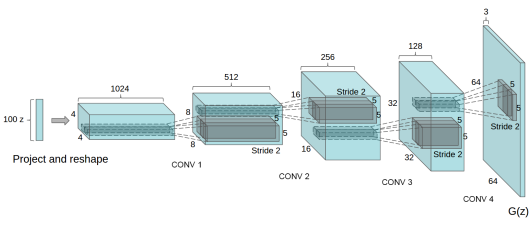
\includegraphics[scale=.7, angle=0]{Files/Generator-Architecture.png}
    \caption[Generator Architecture]{Generator Architecture\cite{DCGAN}}
    \label{fig: DCGAN}
\end{figure}

\section{Training GAN}

Training a GAN is always a tricky part. This work uses DCGAN\cite{DCGAN} as baseline. 